%!TEX root = thesis.tex
\chapter{\acl{HLS}}
\label{chap:hls}
While the benefits of \ac{HLS} in \ac{FPGA} development was already motivated,
this chapter discusses the integration into the ReconOS framework and how it
can be utilized for generating the \ac{OSFSM} and processing logic. Starting
with a detailed introduction into Vivado HLS and its concepts, the resulting
design and implementation decisions for its integration into ReconOS are
discussed. Finally, an evaluation based on the SortDemo application is
presented.

\section{Xilinx Vivado HLS}
Along with the launch of the Vivado tools in 2012, Xilinx releases its
\ac{HLS} tool bought up from AutoESL, formerly known as AutoPilot. It supports
specifications in C, C++ or SystemC and transforms them into synthesizable
\ac{HDL} code. This allows the usage of Vivado \ac{HLS} together with the
Vivado and the ISE implementation tools and simplifies an integration into
ReconOS, currently supporting only the ISE tools. The efficiency of the
generated RTL design in terms of performance and resource utilization depends
hardly on the implementation of the developer and its optimizations for
\ac{HLS}. However, Vivado HLS is able to synthesize nearly every description
into working \ac{HDL} code and several case studies \citep{SWL13,OCC14} have
proven its feasibility for different applications.

\subsection{Toolflow}
While C-style languages are not made for representing hardware, they lack of
according language constructs describing, for example I/O ports or arbitrary
precision data types. Therefore, Vivado HLS introduces a set of conventions,
directives and libraries to retrofit missing, but required features. The
typical \ac{HLS} toolflow as illustrated in figure \ref{fig:hls_flow} takes
the main input files for C-synthesis and C-simulation and generates a
synthesizable \ac{RTL} implementation, together with a set of reports for
analysis of the generated hardware.
\begin{figure}[tb]
	\centering
	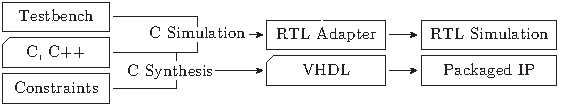
\includegraphics{../figures/hls_flow}
	\caption{The typical Vivado HLS flow \citep[adapted from][]{ug902}}
	\label{fig:hls_flow}
\end{figure}

The primary input for Vivado \ac{HLS} consists out of C functions implemented
in C or C++. Each function synthesizes into a block in the \ac{RTL}
implementation, resulting in a hierarchy of modules representing the hierarchy
of original sub-functions in a one-to-one correspondence. Thereby, a single
function must be specified as the top-level function. Its arguments are
synthesized into top-level \ac{RTL} I/O ports, including automatically
generates clock and control signals. While \ac{HLS} tries to generate an
optimal implementation based on the default behavior, constraints and
directives can be used to control the translation process and to generate
different variants of the same C code. For example \lstinline{HLS UNROLL}
directly influences the synthesis of loops, while clock constraints or target
hardware settings indirectly influence the scheduling and binding phase.
Directives can either be specified in a dedicated file or inline using the the
\lstinline{#pragma} syntax.

Out of the C specifications, directives and constraints, Vivado \ac{HLS}
generates the final \ac{RTL} logic in \ac{VHDL} or Verilog and packs it into
an \ac{IP} for later use with other tools in the Xilinx design flow. To verify
the design and correctness of the implementation, a tesbench allows to execute
and debug the code in a C simulation and provides a C/RTL cosimulation to
compare the results of the software and hardware simulation.

\subsection{Fundamentals}
To write efficient C code for hardware synthesis, understanding the principles
of \ac{HLS} and how the C code is translated into an equivalent \ac{RTL}
implementation is fundamental. Vivado \ac{HLS} follows several phases, namely
scheduling, binding and control logic extraction. Firstly, the control- and
datapaths specified by the program's operations and conditional statements are
extracted and translated into an internal representation. Based on these
information, Vivado HLS performs scheduling, binding and control logic
extraction. Scheduling determines, based on the length of a clock cycle and
timing information for the targeted \ac{FPGA}, which operations are scheduled
in a specific clock cycle. For example, a slower clock frequency allows to
complete more operations in a single clock cycle, while a slower \ac{FPGA}
causes operations to be implemented as multicycle resources. Each of the
scheduled operations is then assigned to a hardware resource in the binding
phase. Finally, the required interfaces for the different \ac{RTL} entities
are synthesized and the control logic is implemented by a \ac{FSM} that
sequences the operations in the \ac{RTL} design.

To illustrate the different phases, listing \ref{lst:hls_code} sketches an
algorithm implemented in C. 
\begin{lstlisting}[
	language=C,
	caption={Scheduling and binding example},
	label={lst:hls_code},
	morekeywords={uint32,uint8},
	float=tb
]
void foo(int in[3], char a, char b, char c, int out[3]) {
	int x,y;
	for(int i = 0; i < 3; i++) {
		x = in[i];
		y = a*x + b + c;
		out[i] = y;
	}
}
\end{lstlisting}
It calculates the sum of operands out of an array and stores the results back
in memory. To simplify the example for the scheduling and binding phase,
consider only line 5, containing a multiplication and two additions. Figure
\ref{fig:hls_sb} shows the corresponding scheduling generated by Vivado
\ac{HLS}.
\begin{figure}[tb]
	\centering
	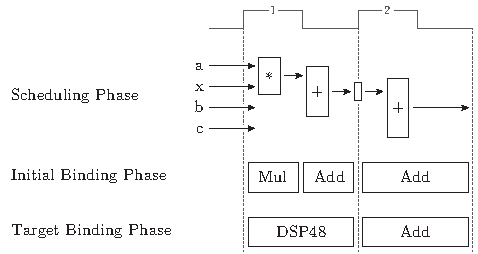
\includegraphics{../figures/hls_sb}
	\caption{Scheduled operations for \lstinline{a*x + b + c}}
	\label{fig:hls_sb}
\end{figure}
Since all three operations cannot be finished within a single clock cycle,
they are split up and executed sequentially. The multiplication and first
addition is scheduled in the first clock cycle, while the second addition is
postponed to the second clock cycle, processing the result of the previous
calculation stored in a register. After scheduled all operations, each one is
assigned to a hardware resource during binding. In the initial phase, each
operation is implemented as combinational logic, while the target phase
optimizes the initial binding by utilizing special resources available on the
target \ac{FPGA}. In this example, instead of implementing the multiplication
and first addition in combinational logic, a \ac{DSP} resources is
instantiated.

After the operations are scheduled and assigned to specific hardware
resources, the control logic needs to be extracted and implemented. Figure
\ref{fig:hls_c} shows the necessary control logic for the example code in
listing \ref{lst:hls_code}.
\begin{figure}[tb]
	\centering
	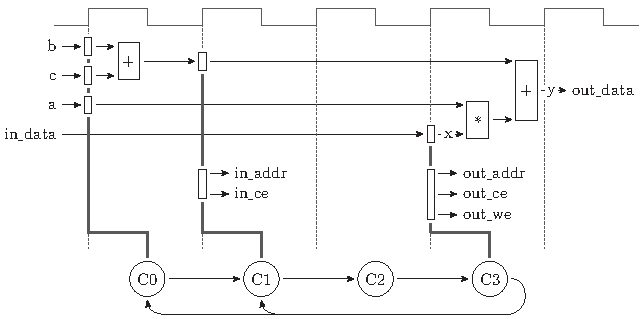
\includegraphics{../figures/hls_c}
	\caption{Extracted control logic for example algorithm}
	\label{fig:hls_c}
\end{figure}
It executes the scheduled operations of the loop body three times, controls
when registers store data and setups the appropriate control signals. Since
the addition of \lstinline{b} and \lstinline{c} needs to be executed only
once, Vivado \ac{HLS} automatically moves it outside of the loop into state C0
and stores the result in a register, reused in state C3. To execute the loop
exactly three times, the \ac{FSM} also manages a counter, incremented each
time it reaches state C1. Since the interface synthesis, explained later,
implements the top-level arguments \lstinline{in} and \lstinline{out} as block
\ac{RAM} interfaces, the control logic generates the according address and
enable signals and respects the required timing by introducing the delay state
C2. During execution, the full sequence of states results in C0, C1, C2, C3, C1, C2, C3, C1, C2, C3, C0.


%A the example code in listing \ref{lst:hls_if}, including two inputs
%\lstinline{in0} and \lstinline{in1}, a pointer \lstinline{sum} and a return
%value.
%\begin{lstlisting}[
%	language=C,
%	caption={Interface specification example},
%	label={lst:hls_if},
%	morekeywords={uint32},
%	float=tb
%]
%uint32 sum(uint32 in0, uint32 in1, uint32 *sum) {
%	*sum = in0 + in1 + *sum;
%	return in0 + in1;
%}
%\end{lstlisting}
Besides the control logic itself, the last synthesis phase also includes the
interface synthesis, generating I/O ports for the top-level entity and
internal ports for communication between the different sub-blocks. Applying
the default interface synthesis settings to the example in listing
\ref{lst:hls_code} results in an interface as shown in figure
\ref{fig:hls_if}. It consists out of clock and reset ports
\lstinline{ap_clk} and \lstinline{ap_rst}, block-level interfaces
\lstinline{ap_start}, \lstinline{ap_done}, \lstinline{ap_idle} and
\lstinline{ap_ready}, and port-level interfaces for the top-level arguments
\lstinline{a}, \lstinline{b}, \lstinline{c}, \lstinline{in} and
\lstinline{out}.
\begin{figure}[tb]
	\centering
	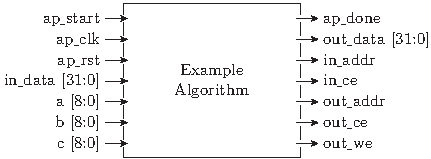
\includegraphics{../figures/hls_if}
	\caption{Generated interface with default settings}
	\label{fig:hls_if}
\end{figure}
The block-level interfaces control the \ac{IP} by allowing the block to start
processing or indicating, whether it is ready to accept data, is idle or has
completed operation. Besides the block-level interfaces generated
independently from any arguments specified by the user, the port-level
interfaces are generated depending on the type of the argument and its usage.
Input pass-by-value arguments and pointers are synthesized as wire ports
without any handshaking signals and must be held valid during operation until
they are read. Arrays are assumed to be modeled as block \acp{RAM} and are
implemented accordingly. When used as top-level arguments, synthesis does not
infer a block \ac{RAM} directly, but generates ports to access a block ram
outside of the top-level entity. While the example code does note specify a
return type, Vivado HLS is capable of synthesizing non-pointer types as
regular out wire ports with \lstinline{ap_done} replacing the typically
implemented valid signal.

While the default settings generate basic block-level ports sufficient for
many applications, Vivado HLS also supports more sophisticated protocols like
\ac{FIFO} or \ac{AXI} interfaces. Since a ReconOS thread is connected via
the \ac{FIFO} based \ac{OSIF} and \ac{MEMIF} interfaces, these advanced port
protocols are highly relevant for an \ac{HLS} integration. However, more
complex protocols do not map sufficiently to primitive datatypes. A pointer
dereferenced sequentially can be used to model a \ac{FIFO} interface, but
reaches its limits for an infinite stream. For these kind of applications,
Xilinx provides a streaming library, implementing the template class
\lstinline{hls::stream}. It guarantees sequential access via blocking and non-
blocking \lstinline{read} and \lstinline{write} methods and, by default, maps
to a \ac{FIFO} interface when used as a top-level argument. Unfortunately, the
co-simulation feature of Vivado HLS does not support streaming datatypes as
arguments of the top-level function, making an external \ac{RTL}-simulator and
a user-created \ac{HDL} testbench necessary.

\section{ReconOS Integration}
Knowing Vivado HLS' fundamental concepts and design flows allows to
investigate an integration into ReconOS, to simplify the development of
hardware threads and open the framework to a broader range of developers. This
includes a way to specify the thread's implementation, including the
processing logic and \ac{OSFSM}, as well as a seamless integration into the
existing toolchain. While the processing logic itself is completely user
defined and only limited by general restrictions of Vivado HLS, the structure
of the \ac{OSFSM} and the thread's external interfaces are prescribed by the
ReconOS framework. These specifications must be respected and generated
accordingly. For convenient use, the existing ReconOS package functions for
\ac{OS} calls and memory access should be adapted to provide a unified
programming interface for all thread descriptions. Especially, the blocking
semantics must be preserved and correctly synthesized. Additionally, an
automatically generated software implementation out of the \ac{HLS}
description would be desirable, especially against the background of
self-adaptive, reconfigurable systems.

\subsection{Interface Description}
A ReconOS hardware thread must implement a fixed set of interfaces to be
connected to the different components of the system. As illustrated in figure
\ref{fig:hwt_if_o} \todo{update signal}, these include the two bidirectional
\ac{FIFO} based \ac{OSIF} and \ac{MEMIF} interfaces, as well as clock, reset
and interrupt signals.
\begin{figure}
	\centering
	\begin{subfigure}{10.2cm}
		\centering
		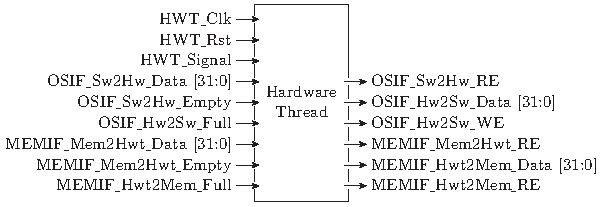
\includegraphics{../figures/hwt_if_o}
		\caption{Required interface}
		\label{fig:hwt_if_o}
	\end{subfigure}
	\par\bigskip
	\begin{subfigure}{10.2cm}
		\centering
		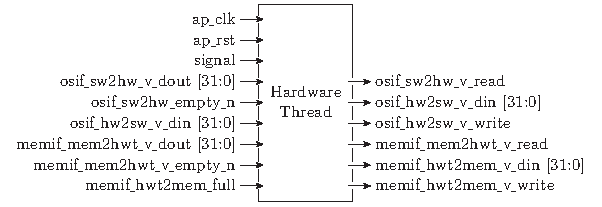
\includegraphics{../figures/hwt_if_h}
		\caption{Interface inferred by Vivado HLS}
		\label{fig:hwt_if_h}
	\end{subfigure}
	\caption{Interfaces of hardware thread}
	\label{fig:hwt_if}
\end{figure}
When generating a hardware thread using Vivado HLS, these interfaces must be
generated and accessed accordingly. As stated in the fundamentals section,
Vivado HLS automatically generates ports for clock and reset signals and also
supports \ac{FIFO} top-level ports. However, while clock and reset ports do
not require a certain protocol, the \ac{FIFO} interfaces implemented by the
ReconOS runtime prescribe certain timing and access conventions. As it turned
out, they are fully compatible with the interfaces generated by Vivado HLS,
making it possible to model the \ac{OSIF} and \ac{MEMIF} as regular \acp{FIFO}
using the \lstinline{hls::stream} class.

Listing \ref{lst:hwt_if_h} show the definition of the top-level function of a
hardware thread, including arguments and directives.
\begin{lstlisting}[
	language=C,
	caption={Exemplary ReconOS thread in C},
	label={lst:hwt_if_h},
	morekeywords={uint32},
	float=tb
]
void thread_entry(hls::stream<uint32> osif_sw2hw,
                  hls::stream<uint32> osif_hw2sw,
                  hls::stream<uint32> memif_hwt2mem,
                  hls::stream<uint32> memif_mem2hwt,
                  hls::stream<bool> sig) {
	#pragma HLS INTERFACE ap_ctrl_none port=return
	#pragma HLS INTERFACE ap_fifo port=osif_sw2hw
	#pragma HLS INTERFACE ap_fifo port=osif_hw2sw
	#pragma HLS INTERFACE ap_fifo port=memif_hwt2mem
	#pragma HLS INTERFACE ap_fifo port=memif_mem2hwt
	#pragma HLS INTERFACE ap_fifo port=sig
	// hardware thread body
}
\end{lstlisting}
The four streaming parameters \lstinline{osif_sw2hw}, \lstinline{osif_hw2sw},
\lstinline{memif_hwt2mem}, \lstinline{memif_mem2hwt} model the \ac{OSIF} and
\ac{MEMIF} interfaces and are forced by the directives in lines 6-9 to be
implemented as \acp{FIFO}. Since the hardware thread does not need the, by
default, generated control signals \lstinline{ap_start}, \lstinline{ap_done},
\lstinline{ap_idle} and \lstinline{ap_ready}, the directive in line 5
instructs Vivado HLS to generate the mandatory clock and reset signals, but
omit the default control ports. Note, that the signal port is mapped as a
\ac{FIFO} interface instead of plain signal. Due to the interface demands of
Vivado HLS, the read of a plain signal with \lstinline{ap_none} protocol would
be scheduled in the first state, independent from its arrangement in the code.
In contrast, mapping the \lstinline{sig} signal as the empty port of a
\ac{FIFO} interface infers the semantics of signal changing during runtime and
allows to check its value via the provided \lstinline{hls::stream} functions.
Furthermore, since \acp{FIFO} are inherently sequential, the read operation is
scheduled in the desired state.

Applying these directives results in an interface as shown in figure
\ref{fig:hwt_if_h}. Comparing it with the required interface of ReconOS
reveals an improper naming of the generated ports. Since Vivado HLS does not
support to specify user defined names, the synthesized top-level model is
wrapped by another entity providing the correct port names and maps the signal
\lstinline{signal} to the empty and data signals of generated \ac{FIFO} ports
and leaves the read signal unconnected.

\subsection{\acs{OSFSM} Specification}
Having the external interfaces modeled using the \lstinline{hls::stream}
class sets out the basis for a hardware thread description in Vivado HLS. A
ReconOS thread is separated into the \ac{OSFSM} and the internal processing
logic as motivated in the introductory chapter. Since the processing logic is
completely application specific and does not use any ReconOS specific
functionality, it is the developers task to implement the desired algorithm
correctly and to interface with the \ac{OSFSM}. However, it is unclear, how
the \ac{OSFSM} can be modeled inside of Vivado HLS. Many \ac{OS} functions
imply a blocking semantic and the ordering of several calls must be preserved.
Since the C code itself has a strongly sequential meaning, it seems to fit
perfectly to model the \ac{OSFSM} structure. Furthermore, all sequential calls
contain access to \ac{FIFO} interfaces, which are inherently sequential and
synthesized accordingly by Vivado HLS. Further data dependencies are also
respected by the synthesis, while independent processing might be executed in
parallel to \ac{OS} calls, speeding up the design.

Listing \ref{lst:osfsm_hls} shows an exemplary ReconOS thread implementing the
\ac{OSFSM} for the SortDemom application.
\begin{lstlisting}[
	language=C,
	caption={Exemplary ReconOS thread in Vivado HLS},
	label={lst:osfsm_hls},
	morekeywords={uint32},
	float=tb
]
#include "reconos_calls.h"
#include "reconos_thread.h"

#include "ap_cint.h"

#define BLOCK_SIZE 2048

THREAD_ENTRY() {
	RAM(uint32, BLOCK_SIZE, ram);

	THREAD_INIT();

	while(1) {
		uint32 addr = MBOX_GET(resources_address);
		MEM_READ(addr, ram, BLOCK_SIZE * 4);

		sort_bubble(ram);

		MEM_WRITE(ram, addr, BLOCK_SIZE * 4);
		MBOX_PUT(resources_acknowledge, addr);
	}
}
\end{lstlisting}
It executes several \ac{OS} calls, accesses the memory and calls the internal
processing logic. While the ReconOS \ac{VHDL} package includes procedures
implementing a nested state machine to access the external interfaces and
emulate blocking calls, Vivado HLS does not allow to interface with external
\ac{HDL} libraries. Therefore, all ReconOS functions were implemented inside
of Vivado HLS, for example \lstinline{MBOX_GET} or \lstinline{MEM_READ}. Even
if these calls look like regular function calls, they are realized as
preprocessor macros due to the semantics of C functions in Vivado HLS. A
function represents a separate module in the synthesized \ac{RTL} design,
which is reasonable for processing logic like the \lstinline{sort_bubble}
function, but not meaningful here. Listing \ref{lst:call_mbox} shows exemplary
the implementation of \lstinline{MBOX_GET}.
\begin{lstlisting}[
	language=C,
	caption={Implementation of \lstinline{MBOX_GET}},
	label={lst:call_mbox},
	morekeywords={uint32},
	float=tb
]
#define MBOX_GET(p_handle)(\
	stream_write(osif_hw2sw, OSIF_CMD_MBOX_GET),\
	stream_write(osif_hw2sw, p_handle),\
	stream_read(osif_sw2hw))
\end{lstlisting}
It consists out of two writes to the outgoing \ac{OSIF}, followed by a read
from the incoming \ac{OSIF} and corresponds directly to the \ac{VHDL}
implementation. It should be noted, that all \ac{FIFO} accesses are performed
in a blocking manner and synthesized by Vivado HLS accordingly. When analyzing
the design as shown in figure \ref{fig:osfsm_a}, the sequential execution
becomes apparent. Rows 5, 7 and 9 represent the \ac{FIFO} access, scheduled in
three different states, sequentially executed after each other.
\begin{figure}[tb]
	\centering
	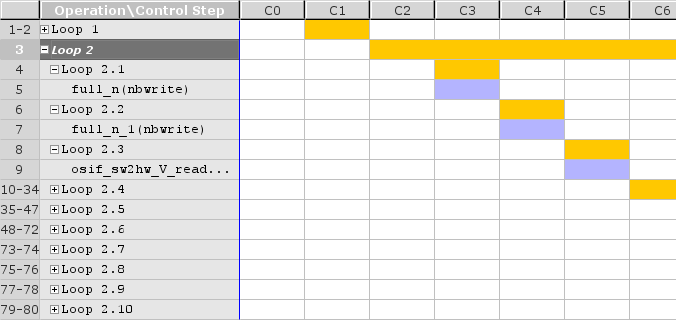
\includegraphics[width=10cm]{../figures/osfsm_a}
	\caption{Analysis of synthesized \acs{OSFSM}}
	\label{fig:osfsm_a}
\end{figure}
Furthermore, data dependency introduced by the \ac{OS} calls are preserved.
For example, the internal processing logic accesses the on-chip ram after the
initialization by \lstinline{MEM_READ} with the unsorted data. Vivado HLS
schedules these accesses to guarantee the right order of execution. However,
unlike in a hand-coded implementation, the processing logic might interleave
with the \ac{OS} calls whenever possible.

Besides the ReconOS calls itself, the library files include several macros to
reduce the complexity and provide a convenient \ac{API} to the developer. For
example, the macro \lstinline{THREAD_ENTRY} expands to the function prototype
sketched in listing \ref{lst:hwt_if_h}, defining the \ac{OSIF} and \ac{MEMIF}
interfaces as top-level arguments and the \lstinline{RAM} macro wraps the
instantiation of an on-chip \ac{RAM}.

Utilizing the inherently sequential meaning of C code allows a convenient
specification of the \ac{OSFSM} in Vivado HLS, similar to a software
specification. In fact, the same C code used to synthesize custom hardware can
also be executed on the \ac{CPU}. Having all hardware specific functionality
wrapped inside of the ReconOS macros allows to generate a corresponding
implementation in software. Instead of writing into the
\acp{FIFO} and delegating the \ac{OS} calls to the delegate threads, the
appropriate system calls are executed directly and memory accesses are mapped
to pointer operations.

\subsection{Toolchain Integration}
To provide a convenient development flow, the Vivado HLS tool needs to be
integrated into the existing ReconOS toolflow. It takes the \ac{VHDL}
implementation provided by the developer and packs it into an \ac{IP} core
using a predefined template. The \ac{IP} core itself is then integrated into
the reference design template, resulting in a ready-to-build EDK project. All
these steps are automated in the \ac{RDK}, providing an extendable and loosely
coupled architecture implemented in Python. Each functionality is encapsulated
into an independent script, utilizing runtime functionality like a template
generator or methods for file operations.

Since Vivado HLS synthesizes an \ac{RTL} representation in \ac{VHDL}, it can
be integrated into the existing toolflow seamlessly, by prepending the
additional \ac{HLS} step before the \ac{IP} packaging as illustrated in figure
\ref{fig:rdk}.
\begin{figure}
	\centering
	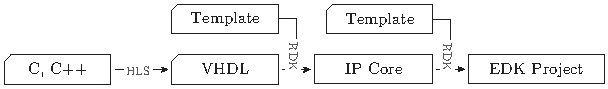
\includegraphics{../figures/rdk}
	\caption{Adopted toolflow for Vivado HLS}
	\label{fig:rdk}
\end{figure}
To automate the process of executing Vivado HLS and generating the \ac{RTL}
implementation, Xilinx includes a \ac{Tcl} interpreter combined with a batch
operation mode. Listing \ref{lst:hls_tcl} shows the \ac{Tcl} template used for
synthesizing the developer's source code.
\begin{lstlisting}[
	language=TCL,
	caption={\acs{Tcl} template for Vivado HLS},
	label={lst:hls_tcl},
	float=tb
]
<<reconos_preproc>>

open_project hls
set_top rt_imp
add_files reconos_calls.h
add_files reconos_thread.h
add_files [ glob *.cpp ]
open_solution sol
set_part {<<PART>>}
create_clock -period <<CLKPRD>> -name default
source directives.tcl
csynth_design
exit
\end{lstlisting}
It adds the source and directive files to the project, configures the
appropriate target \ac{FPGA} and clock settings, synthesizes the design and
exits Vivado HLS. The resulting \ac{VHDL} implementation is then processed
similarly to a regular \ac{VHDL} specification provided by the user, except
that the generated top-level module is wrapped by an additional entity to
compensate the improper port naming.

Beside the generation of a hardware description, the toolchain also
supports the generation of a software implementation out of the \ac{HLS}
specification. As stated earlier, it represents valid C code and can be
compiled without any changes by using the adopted header file
\lstinline{reconos_calls_c.h}, defining the ReconOS macros for usage in
software.

The seamless integration of Vivado HLS into the ReconOS toolflow provides a
convenient development environment. Implementing a thread in Vivado HLS
requires the developer to setup the source files in the \lstinline{hls}
directory of the thread's sources, specify the appropriate option
\lstinline{hls} as \lstinline{HwSource} or \lstinline{SwSource} in the project
file and export the design.

\section{Evaluation}
Since many case studies in the literature demonstrated the advantages of
Vivado HLS in terms of design time and performance, the integration into
ReconOS promises similar results. Additionally, it provides the advantages of
a convenient programming model for hybrid multi-core systems at system level.
To evaluate the particular benefits and drawbacks, the well-known SortDemo was
implemented in Vivado HLS with different optimizations and compared to the
classical, hand- coded \ac{VHDL} implementation in terms of performance and
area-consumption.

Before considering the resulting performance metrics, the development process
should be taken into account. The SortDemo threads implement a rather
inefficient bubble sort algorithm. While the custom \ac{VHDL} specification
was developed by experienced hardware designers within weeks, the \ac{HLS}
implementation required significantly less effort. The bubble sort algorithm
can be implemented in C by even unpracticed developers and verified very
easily. Compiling and executing the \ac{HLS} implementation on a \ac{CPU}
allows dramatically simplified testing and debugging without complex \ac{RTL}
simulations or time consuming implementation delays. Already for this
uncomplex application, Vivado HLS offered a significant advantage in terms of
error rate, development time and required programmer skills. Together with the
highly accepted multithread programming model, this lowers the entry barrier
and allows even programmers totally unfamiliar with \acp{HDL} to benefit from
a hardware accelerated application.

Table \ref{tab:hls_util} shows the resource utilization of the two
implementations on a ZedBoard evaluation board.
%+-----------------------------------------------------------+--------------+
%| Impl  | Slices* | Slice Reg | LUTs  | LUTRAM | BRAM | DSP | Time         |
%+-----------------------------------------------------------+--------------+
%| VHDL  | 182     | 352       | 501   | 0      | 2    | 0   | 104.940117ms |
%| HLS   | 271     | 539       | 723   | 0      | 2    | 0   | 84.062141ms  |
%+-----------------------------------------------------------+--------------+
\begin{table}
	\scriptsize
	\centering
	\captionabove{Resource utilization of \acs{VHDL} and \acs{HLS}}
	\label{tab:hls_util}
	\begin{tabular}{lcccc}
	\hline
	\textbf{Type} & \textbf{Slices} & \textbf{Slice Reg} & \textbf{LUTs} & \textbf{BRAM}\\
	\hline
	\ac{VHDL} & 182 & 352 & 501 & 2\\
	\ac{HLS} & 271 & 539 & 723 & 2\\
	\hline
	\end{tabular}
\end{table}
The thread written in \ac{VHDL} has an overall lower resource utilization.
However, it is noticeably slower in terms of execution time. While the
\ac{HLS} implementation takes $\SI{84.06}{\milli\second}$ in average over 1024
iterations to sort a block of 2048 words, the hand-coded variant needs
$\SI{104.94}{\milli\second}$ in the same average and is, therefore, around
20\% slower. Insofar, the higher resource utilization is acceptable and not
necessarily a drawback, in particular when considering the implementation
effort taken. Note, that both implementations are significantly faster than
the according software implementation taking $\SI{216.32}{\milli\second}$ in
average for a single block.

Further optimizations like loop unrolling or deep pipelining cannot be applied
in this application. The overall performance is restricted by the local
\ac{RAM}, providing only sequential access to the user data. A distributed
implementation of the \ac{RAM} resources would eliminate that bottleneck, but
is limited by available resources and not feasible for this application. Even
with a reduced block size of 128 word, a distributed \ac{RAM} would consume
around 75\% of the ZedBoard's \acp{LUT}.